% -*- coding:utf-8 -*-
% LATEX PREAMBLE --- needs to be imported manually
\documentclass[12pt]{article}
% \special{papersize=3in,5in}

\usepackage[utf8]{inputenc}
\usepackage{amssymb,amsmath,amsthm}
\usepackage{graphicx}
\pagestyle{empty}
\setlength{\parindent}{0in}

\newcommand{\detail}[1]{{\LARGE#1\par}~}
\newcommand{\refs}[1]{{\LARGE\textit{References: }#1\par}\hfill.}
\newcommand*{\abs}[1]{\left\vert#1\right\vert}
\newcommand{\lgmth}[1]{\begingroup\LARGE\[#1\]\endgroup}

%%% commands that do not need to imported into Anki:
\usepackage{mdframed}
\newcommand*{\tags}[1]{\paragraph{tags: }#1\bigskip}
\newcommand*{\xfield}[1]{\begin{mdframed}[font=\sffamily\LARGE]\centering #1\end{mdframed}\bigskip}
\newenvironment{field}{}{}
\newcommand*{\xplain}[1]{\begin{mdframed}\texttt{#1}\end{mdframed}\bigskip}
\newenvironment{plain}{\ttfamily}{\par}
\newenvironment{note}{}{}
% END OF THE PREAMBLE

% Integral dx
\newcommand{\dx}{\mathrm{d}x}

%
% Various Helper Commands
%

% For derivatives
\newcommand{\deriv}[1]{\frac{\mathrm{d}}{\mathrm{d}x} (#1)}

% For partial derivatives
\newcommand{\pderiv}[2]{\frac{\partial}{\partial #1} (#2)}


% Alias for the Solution section header
\newcommand{\solution}{\textbf{\large Solution}}

% Probability commands: Expectation, Variance, Covariance, Bias
\newcommand{\E}{\mathrm{E}}
\newcommand{\Var}{\mathrm{Var}}
\newcommand{\Cov}{\mathrm{Cov}}
\newcommand{\Bias}{\mathrm{Bias}}

% Formatting commands:

\newcommand{\mt}[1]{\ensuremath{#1}}
\newcommand{\nm}[1]{\textrm{#1}}

\newcommand\bsc[2][\DefaultOpt]{%
  \def\DefaultOpt{#2}%
  \section[#1]{#2}%
}
\newcommand\ssc[2][\DefaultOpt]{%
  \def\DefaultOpt{#2}%
  \subsection[#1]{#2}%
}
\newcommand{\bgpf}{\begin{proof} $ $\newline}

\newcommand{\bgeq}{\begin{equation*}}
\newcommand{\eeq}{\end{equation*}}	

\newcommand{\balist}{\begin{enumerate}[label=\alph*.]}
\newcommand{\elist}{\end{enumerate}}

\newcommand{\bilist}{\begin{enumerate}[label=\roman*)]}	

\newcommand{\bgsp}{\begin{split}}
% \newcommand{\esp}{\end{split}} % doesn't work for some reason.

\newcommand\prs[1]{~~~\textbf{(#1)}}

\newcommand{\lt}[1]{\textbf{Let: } #1}
     							   %  if you're setting it to be true
\newcommand{\supp}[1]{\textbf{Suppose: } #1}
     							   %  Suppose (if it'll end up false)
\newcommand{\wts}[1]{\textbf{Want to show: } #1}
     							   %  Want to show
\newcommand{\as}[1]{\textbf{Assume: } #1}
     							   %  if you think it follows from truth
\newcommand{\bpth}[1]{\textbf{(#1)}}

\newcommand{\step}[2]{\begin{equation}\tag{#2}#1\end{equation}}
\newcommand{\epf}{\end{proof}}

\newcommand{\dbs}[3]{\mt{#1_{#2_#3}}}

\newcommand{\sidenote}[1]{-----------------------------------------------------------------Side Note----------------------------------------------------------------
#1 \

---------------------------------------------------------------------------------------------------------------------------------------------}

% Analysis / Logical commands:

\newcommand{\br}{\mt{\mathbb{R}} }       % |R
\newcommand{\bq}{\mt{\mathbb{Q}} }       % |Q
\newcommand{\bn}{\mt{\mathbb{N}} }       % |N
\newcommand{\bc}{\mt{\mathbb{C}} }       % |C
\newcommand{\bz}{\mt{\mathbb{Z}} }       % |Z
\newcommand{\bi}{\bnm{\mathbb{R}}{\mathbb{Q}}} % |Irrationals 

\newcommand{\ep}{\mt{\epsilon} }         % epsilon
\newcommand{\fa}{\mt{\forall} }          % for all
\newcommand{\afa}{\mt{\alpha} }
\newcommand{\bta}{\mt{\beta} }
\newcommand{\dta}{\mt{\delta} }
\newcommand{\mem}{\mt{\in} }
\newcommand{\exs}{\mt{\exists} }

\newcommand{\es}{\mt{\emptyset} }        % empty set
\newcommand{\sbs}{\mt{\subset} }         % subset of
\newcommand{\fs}[2]{\{\uw{#1}{1}, \uw{#1}{2}, ... \uw{#1}{#2}\}}

\newcommand{\lra}{ \mt{\longrightarrow} } % implies ----->
\newcommand{\rar}{ \mt{\Rightarrow} }     % implies -->
\newcommand{\lba}{ \mt{\longmapsto} }     % element maps to |--->

\newcommand{\lla}{ \mt{\longleftarrow} }  % implies <-----
\newcommand{\lar}{ \mt{\Leftarrow} }      % implies <--

\newcommand{\av}[1]{\mt{|}#1\mt{|}}  % absolute value

\newcommand{\prn}[1]{(#1)}
\newcommand{\bk}[1]{\{#1\}}
\newcommand{\abk}[1]{\mt{\langle}#1\mt{\rangle}}

\newcommand{\ps}{\mt{+} }
\newcommand{\ms}{\mt{-} }

\newcommand{\ls}{\mt{<} }
\newcommand{\gr}{\mt{>} }

\newcommand{\lse}{\mt{\leq} }
\newcommand{\gre}{\mt{\geq} }

\newcommand{\eql}{\mt{=} }

\newcommand{\pr}{\mt{^\prime} } 		   % prime (i.e. R')
\newcommand{\uw}[2]{#1\mt{_{#2}}}
\newcommand{\uf}[2]{#1\mt{^{#2}}}
\newcommand{\frc}[2]{\mt{\frac{#1}{#2}}}
\newcommand{\lmti}[1]{\mt{\displaystyle{\lim_{#1 \to \infty}}}}
\newcommand{\limt}[2]{\mt{\displaystyle{\lim_{#1 \to #2}}}}

\newcommand{\bnm}[2]{\mt{#1\setminus{#2}}}
\newcommand{\bnt}[2]{\mt{\textrm{#1}\setminus{\textrm{#2}}}}

\newcommand{\urng}[2]{\mt{\bigcup_{#1}^{#2}}}
\newcommand{\nrng}[2]{\mt{\bigcap_{#1}^{#2}}}
\newcommand{\nck}[2]{\mt{{#1 \choose #2}}}

     							   
\newcommand{\eqn}[1]{\[#1\]}
\newcommand{\splt}[1]{\begin{split}#1\end{split}}

\newcommand{\infy}{\mt{\infty} }
\newcommand{\unn}{\mt{\cup} }
\newcommand{\inn}{\mt{\cap} }
\newcommand\tab[1][1cm]{\hspace*{#1}}
\newcommand{\rln}{ \mt{\sim} }
\newcommand{\dvd}{ \mt{\vert} }
\newcommand{\ndvd}{ \mt{\not\vert} }
\newcommand{\eqw}{ \mt{ \equiv } }
\newcommand{\lcg}{ \mt{\gamma} }

\newcommand{\edp}{\mt{\bigoplus} }

\newcommand{\wit}[1]{\mt{\widetilde{#1}}}

\newcommand{\mxc}[5]{ % Matrix Column: entry entry entry entry DIMENSION
\underset{#5 \times 1}{
  \begin{bmatrix}
     #1 \\
     #2 \\
     #3 \\
     #4
  \end{bmatrix}
  }
}

\newcommand{\mxr}[5]{ % Matrix Row:    entry entry entry entry DIMENSION
\underset{1 \times #5}{
  \begin{bmatrix}
     #1 & #2 & #3 & #4
  \end{bmatrix}
  }
}

\begin{document}

Joshua Mitchell; MATH 5374; Exercises 11.3, 12.2

\

11.3

\

Take m \eql 50, n \eql 12. Using MATLAB's linspace, define t to be the m vector corresponding to linearly spaced grid points from 0 to 1. Using MATLAB's vander and fliplr, define A to be the m by n matrix associated with least squares fitting on this grid by a polynomial of degree n \ms 1. Take b to be the function cos(4t) evaluated on the grid. Now, calculate and print (to sixteen digit precision) the least squares coefficient vector x by 6 methods:

\begin{enumerate}
  \item Formulation and solution of the normal equations, using MATLAB's backslash.
  \item QR factorization computed by mgs (Ex 8.2)
  \item QR factorization computed by house (Ex 10.2)
  \item QR factorization computed by MATLAB's qr
  \item x \eql A / b in MATLAB.
  \item SVD, using MATLAB's svd
\end{enumerate}

The calculations above will produce six lists of twelve coefficients. In each list, shade with red pen the digits that appear to be wrong (affected by rounding error). Comment on what differences you observe. Do the normal equations exhibit instability? You don't have to explain your observations.

\newpage

\begin{figure}
  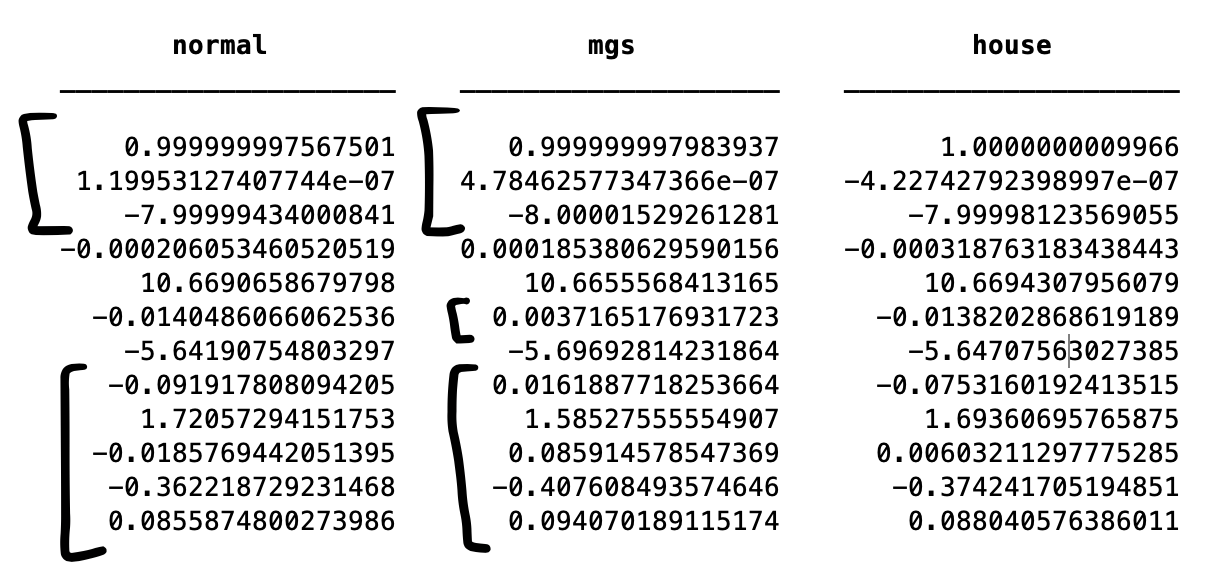
\includegraphics[width=\linewidth]{1131.png}
  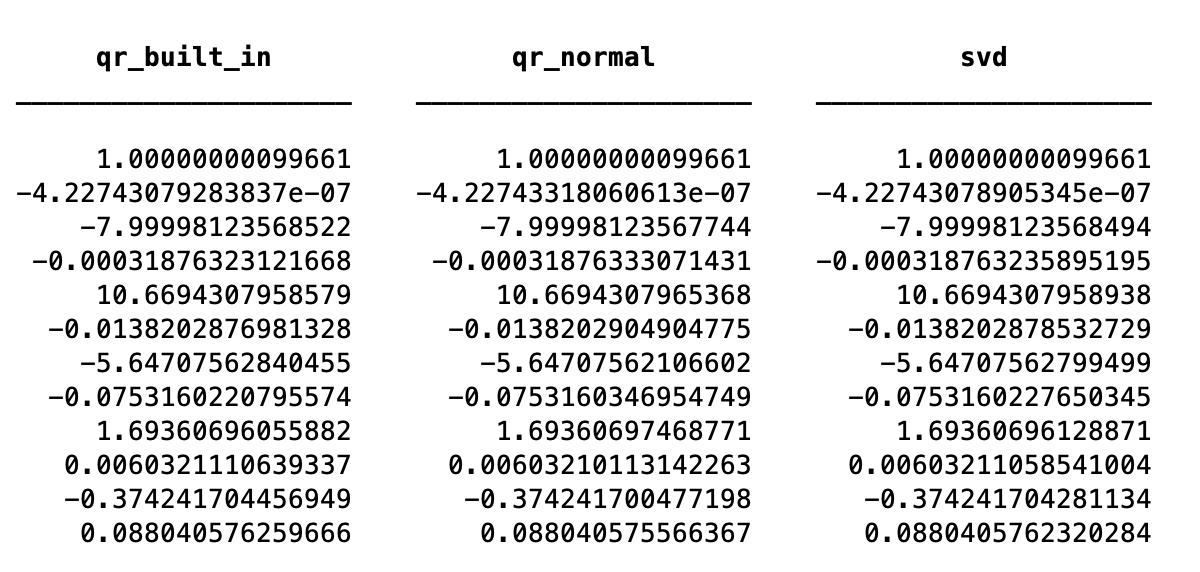
\includegraphics[width=\linewidth]{1132.png}
\end{figure}

\newpage

For the most part, house, SVD, x \eql A / b and MATLAB's built in QR line up pretty well. It's the normal equations and mgs that are noticably wrong (as compared to the other 4). When comparing mgs and normal equations to the other 4, mgs and normal equations are very often wrong on the first significant decimal place, and when they're right on the first, they're wrong by the 3rd or 4th decimal place at the latest.

\

The normal equations definitely exhibit instability (as indicated by MATLAB and this error):

\begin{verbatim}
  Warning: Matrix is close to singular or badly scaled. Results may be inaccurate. RCOND =  3.093573e-17. 
\end{verbatim}

\

12.2

\

In example 11.1 we remarked that polynomial interpolation in equispaced points is ill-conditioned. To illustrate this phenomenon, let \uw{x}{1}, \uw{x}{2}, ..., \uw{x}{n} and \uw{y}{1}, \uw{y}{2}, ..., \uw{y}{m} be n and m equispaced points from -1 to 1, respectively.

\begin{enumerate}
  \item Derive a formula for the m x n matrix A that maps an n-vector of data at \bk{x$_j$} to an m-vector of sampled values \bk{p(y$_j$)}, where p is the degree n \ms 1 polynomial interpolant of the data (see Example 1.1).
  \item Write a program to calculate A and plot $||A||_\infty$ on a semilog scale for n \eql 1, 2, ..., 30, and m \eql 2n \ms 1.
  
  In the continuous limit m \lra \infy, the numbers $||A||_\infty$ are known as Lebesgue constants for equispaced interpolation, which are asymptotic to \uf{2}{n}/(e(n \ms 1) log n) as n \lra \infy.
  
  \item For n \eql 1, 2, ..., 30 and m \eql 2n \ms 1, what is the \infy norm condition number k of hte problem of interpolating the constant function 1? (Use 12.6).
  \item How close is your result for n \eql 11 to the bound implicit in Figure 11.1?
\end{enumerate}


\end{document}